
\section{Handshake circuits}

One of the approaches to design of asynchronous circuits is syntax-directed mapping with 
handshake circuits as an intermediate format. The parse tree of a program source code written in 
a CSP-style \cite{csp} language can be interpreted as a graph of components, connected with communication links
called handshake channels. The components can then be individually mapped to gate-level implementations
with complete circuit derived by implementing the handshake channels with wires.

This approach has been first used by Philips in their Tangram \cite{tangram} design tool
and later made publicly available when the similar free Balsa \cite{balsa} system has been released.

This thesis will be working with Balsa handshake components.

A handshake activation $h$ is said to \emph{enclose} a process $p$ if $p$ can only start after $h$ gets a request and $h$ can get an acknowledgement only after $p$ gets finished.

A \emph{handshake circuit} consists of handshake components which interact by request\slash acknowledgment handshaking 
over communication channels.
Each \emph{handshake component} is specified by a set of ports and a process communicating over those ports.
A \emph{protocol} is assigned to each port, which specifies whether the process initiates the handshakes
over an \emph{active port} or awaits for the other party over a \emph{passive port}. 
It also specifies the direction and size of data transferred during the handshakes.
Each \emph{channel} connects two ports of the same data size with one port being active and the other being passive.
Active input ports and passive output ports are called \emph{pull} ports while the pasive input and active output ports are called \emph{push} ports.

On diagrams used in this thesis we display handshake components with large circles with a process symbol inside
and handshake ports with small circles where filled circle stands for active port and hollow circle stands for passive port.
Channels are displayed as lines between the corresponding ports with the direction of the arrow corresponding to the
direction of data flow.

The defining feature of a handshake component is the process associated with it.
In Balsa there are about fifty types of processes with each having its own behaviour.

An important notion used to describe behaviours is channel \emph{activation}. Activation is a process 
starting with a request being sent from the active port to the passive port and ending with an acknowledgement being sent back.
The behaviour of a channel can be described as activation repeated indefinitely. For data channels activation additionally determines 
the period of time the values on the data wires remain valid.

Processes, including activations, are subject to a notion of \emph{enclosure} to describe temporal relationship between them. 
It is said that a process $p$ is enclosed into a process $q$ when the beginning of $p$ comes after the beginning of $q$ while the end of $p$ comes before the end end of $q$.

\begin{itemize}
\item
$Sequence$ (Fig.~\ref{fig:Sequence-HC}) is a component with three control ports: a passive port $s$ and two active ports $t_1$ and $t_2$.
The behaviour of the component is as follows: each activation on $s$ encloses the process consisting of sequential activation on $t_1$ followed by $t_2$.

\item
$Concur$ (Fig.~\ref{fig:Concur-HC}) is a component with a similar external interface: it has a passive port $s$ and two active ports $t_1$ and $t_2$.
The behaviour is different though: each activation on $s$ for this component encloses activation of $t_1$ and $t_2$ concurrently.

\item
$Sync$ (Fig.~\ref{fig:Sync-HC}) is a component with three control ports: two passive ports $s_1$ and $s_2$ and an active port $t$.
This component ensures enclosure of $t$ into both $s_1$ and $s_2$ by the means of synchronisation between $s_1$ and $s_2$. This component is dual 
to $Concur$ in the sense that they form a no-op when their corresponding ports are connected.

\item
$Call$ (Fig.~\ref{fig:Call-HC}) is another component with three control ports: two passive ports $s_1$ and $s_2$ and an active port $t$.
It differs from Sync in that instead of expecting concurrent activation of both $s_1$ and $s_2$ it only expects one of them to be activated at a time and encloses $t$ into the one which happens.

\item
$BinaryFunc$ (Fig.~\ref{fig:BinaryFunc-HC}) is a component with three pull data ports: a passive port $o$ and two active ports $i_1$ and $i_2$. It is parametrised on width of those ports and on a function it computes. Control-wise it is similar to Concur: it encloses the concurrent activation of $i_1$ and $i_2$ into the activation on $o$.

\item
$CallMux$ (Fig.~\ref{fig:CallMux-HC}) is a component similar to $Call$ with the difference that all of its ports are further extended to $w$-bit pull ports.
Its behaviour is identical from the control point of view, with the additional data being received through $t$ and sent through the activated output port.

\item
$Variable$ (Fig.~\ref{fig:Variable-HC}) is a component with a single input data port $w$, called the write port and a set of passive output data ports $r$, called read ports. 
The component is parameterised on the bit width of the variable $w$, coinciding with the width of the data ports. It is also parameterised on the number of read ports $n$. 
The behaviour  of $Variable$ is to remember the data written with the latest activation of $w$ and to output that data on any activation of a read port $r_i$.
The behaviour is trivial from the control point of view: the only way the ports interact is through the data. However, there is a requirement that the write port activation does not overlap with any of the read port activations.

\item
$While$ (Fig.~\ref{fig:While-HC}) is a component with a passive control port $s$, an active control port $t$ and an active one-bit input data port $c$. Its behaviour is to enclose into the activation on $s$ the following process:
complete a handshake over $c$ to obtain the one-bit data indicating the process activity condition; if this condition holds then activate $t$ and repeat the operations.

\item
$Case$ (Fig.~\ref{fig:Case-HC}) is a component with a passive input data port $i$ and a set of active control ports $t$. It is parameterised by a number of ports $n$, 
the size of the data transferred by $i$ and by a function $f$ mapping $2^{|c|}\rightarrow n$.
The behaviour is to enclose into activation on $i$ with the input code word $d$ an activation of the port $t_{f(d)}$.

\end{itemize}



\begin{figure}
\centering
\subfloat[Sequence\label{fig:Sequence-HC}]{
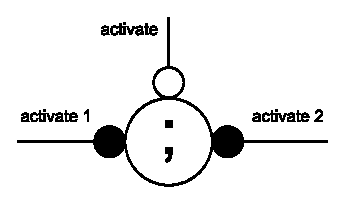
\includegraphics[scale=0.5]{figures/Control/sequence-HC}
} {}
\subfloat[Concur\label{fig:Concur-HC}]{
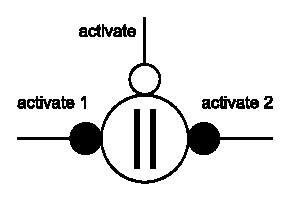
\includegraphics[scale=0.5]{figures/Control/concur-HC}
} {}
\subfloat[Sync\label{fig:Sync-HC}]{

\includegraphics[scale=0.5]{figures/Control/sync-HC}
} {}
\subfloat[Call\label{fig:Call-HC}]{

\includegraphics[scale=0.5]{figures/Control/call-HC}
} {}

\subfloat[BinaryFunc\label{fig:BinaryFunc-HC}]{
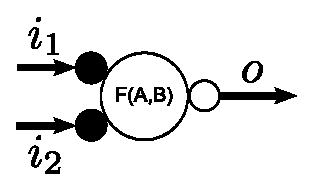
\includegraphics[bb=0bp 0bp 134bp 80bp,scale=0.5]{figures/Data/binaryfunc-HC}
} {}
\subfloat[CallMux\label{fig:CallMux-HC}]{
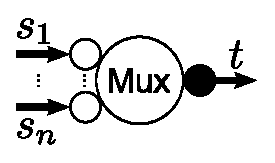
\includegraphics[scale=0.5]{figures/Data/callmux-HC}
} {}
\subfloat[Variable\label{fig:Variable-HC}]{
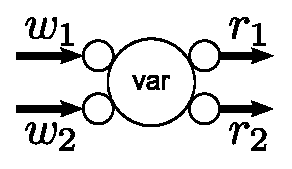
\includegraphics[scale=0.5]{figures/Data/variable-HC}
} {}
\subfloat[While\label{fig:While-HC}]{
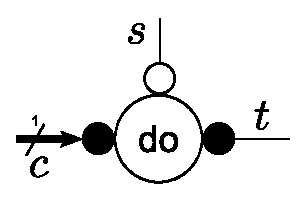
\includegraphics[bb=0bp 0bp 134bp 80bp,scale=0.5]{figures/while-HC}
} {}
\subfloat[Case\label{fig:Case-HC}]{

\includegraphics[scale=0.5]{figures/case-HC}
}

\caption{Handshake components}
\end{figure}

